% appendix/rcuimpl/rcupreempt.tex

\section{Preemptible RCU}
\label{app:rcuimpl:Preemptible RCU}
\OriginallyPublished{Appendix}{app:rcuimpl:Preemptible RCU}{Preemptible RCU}{Linux Weekly News}{PaulEMcKenney2007PreemptibleRCU}

The preemptible RCU implementation is unusual in that
it permits read-side critical
sections to be preempted and to be blocked waiting for locks.
However, it does not handle general blocking
(for example, via the \co{wait_event()} primitive):
if you need that, you should instead use SRCU, which is described in
Appendix~\ref{app:rcuimpl:Sleepable RCU Implementation}.
In contrast to SRCU,
preemptible RCU only permits blocking within primitives that are
both subject to priority inheritance and non-blocking in a
non-\co{CONFIG_PREEMPT} kernel.
This ability to acquire blocking locks and to be preempted within
RCU read-side critical sections is required for the aggressive real-time
capabilities provided by Ingo Molnar's -rt patchset.
However, the initial preemptible RCU implementation~\cite{PaulMcKenney2005d}
had some limitations, including:

\begin{enumerate}
\item	Its read-side primitives cannot be called from within
	non-maskable interrupt (NMI) or systems-management interrupt
	handlers.
\item	Its read-side primitives use both atomic instructions and
	memory barriers, both of which have excessive overhead.
\item	It does no priority boosting of RCU read-side critical
	sections~\cite{PaulEMcKenney2007BoostRCU}.
\end{enumerate}

The new preemptible RCU implementation that accepted into the 2.6.26
Linux kernel
removes these limitations, and this appendix describes its design,
serving as an update to the LWN article~\cite{PaulEMcKenney2007PreemptibleRCU}.
However, please note that this implementation was replaced with a faster
and simpler implementation in the 2.6.32 Linux kernel.
This description nevertheless remains to bear witness to the most complex
RCU implementation ever devised.

\QuickQuiz{}
	Why is it important that blocking primitives
	called from within a preemptible-RCU read-side critical section be
	subject to priority inheritance?
\QuickQuizAnswer{
	Because blocked readers stall RCU grace periods,
	which can result in OOM.
	For example, if a reader did a \co{wait_event()} within
	an RCU read-side critical section, and that event never occurred,
	then RCU grace periods would stall indefinitely, guaranteeing that
	the system would OOM sooner or later.
	There must therefore be some way to cause these readers to progress
	through their read-side critical sections in order to avoid such OOMs.
	Priority boosting is one way to force such progress, but only if
	readers are restricted to blocking such that they can be awakened via
	priority boosting.

	Of course, there are other methods besides priority inheritance
	that handle the priority inversion problem, including priority ceiling,
	preemption disabling, and so on.
	However, there are good reasons why priority inheritance is the approach
	used in the Linux kernel, so this is what is used for RCU.
} \QuickQuizEnd

\QuickQuiz{}
	Could the prohibition against using primitives
	that would block in a non-\co{CONFIG_PREEMPT} kernel be lifted,
	and if so, under what conditions?
\QuickQuizAnswer{
	If testing and benchmarking demonstrated that the
	preemptible RCU worked well enough that classic RCU could be dispensed
	with entirely, and if priority inheritance was implemented for blocking
	synchronization primitives
	such as \co{semaphore}s, then those primitives could be
	used in RCU read-side critical sections.
} \QuickQuizEnd

\subsection{Conceptual RCU}
\label{app:rcuimpl:Conceptual RCU}

Understanding and validating an RCU implementation is much easier given
a view of RCU at the lowest possible level.
This section gives a very brief overview of the
most basic concurrency requirements that an RCU implementation must
support.
For more detail, please see
Section~\ref{sec:defer:RCU Fundamentals}.

RCU implementations must obey the following rule: if any
statement in a given RCU read-side critical section precedes a
grace period, then all statements in that RCU read-side critical
section must complete before that grace period ends.

\begin{figure}[htb]
\centering
\resizebox{3in}{!}{\includegraphics{appendix/rcuimpl/GracePeriodBad}}
\caption{Buggy Grace Period From Broken RCU}
\label{app:rcuimpl:Buggy Grace Period From Broken RCU}
\end{figure}

This is illustrated by
Figure~\ref{app:rcuimpl:Buggy Grace Period From Broken RCU},
where time advances from left to right.
The red ``Removal'' box represents the update-side critical section that
modifies the RCU-protected data structure, for example, via
\co{list_del_rcu()}; the large yellow ``Grace Period'' box
represents a grace period (surprise!) which might be invoked via
\co{synchronize_rcu()}, and the green ``Reclamation'' box
represents freeing the affected data element,
perhaps via \co{kfree()}.
The blue ``Reader'' boxes each represent an RCU read-side critical section,
for example, beginning with \co{rcu_read_lock()} and ending with
\co{rcu_read_unlock()}.
The red-rimmed ``Reader'' box is an example of an illegal situation:
any so-called RCU implementation that permits a read-side critical section
to completely overlap a grace period is buggy, since the updater might
free up memory that this reader is still using.

So, what is the poor RCU implementation to do in this situation?

\begin{figure}[htb]
\centering
\resizebox{3in}{!}{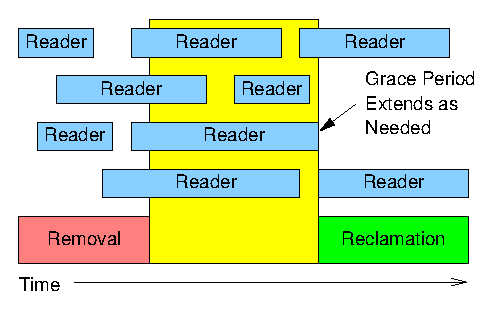
\includegraphics{appendix/rcuimpl/GracePeriodGood}}
\caption{Good Grace Period From Correct RCU}
\label{app:rcuimpl:Good Grace Period From Correct RCU}
\end{figure}

It must extend the grace period, perhaps as shown in
Figure~\ref{app:rcuimpl:Good Grace Period From Correct RCU}.
In short, the RCU implementation must ensure that any
RCU read-side critical sections in progress at the start of a given grace
period have completely finished, memory operations and all, before that
grace period is permitted to complete.
This fact allows RCU validation to be extremely focused: simply demonstrate
that any RCU read-side critical section in progress at the beginning of
a grace period must terminate before that grace period ends, along with
sufficient barriers to prevent either the compiler or the CPU from undoing
the RCU implementation's work.

\subsection{Overview of Preemptible RCU Algorithm}
\label{app:rcuimpl:Overview of Preemptible RCU Algorithm}

This section focuses on a specific implementation of preemptible RCU.
Many other implementations are possible, and are described
elsewhere~\cite{PaulEMcKenney2006b,PaulMcKenney05b}.
This article focuses on this specific implementation's
general approach, the data structures,
the grace-period state machine, and a walk through the read-side primitives.

\subsubsection{General Approach}
\label{app:rcuimpl:General Approach}

\begin{figure}[htb]
\centering
\resizebox{3in}{!}{\includegraphics{appendix/rcuimpl/RCUpreemptListsCompare}}
\caption{Classic vs. Preemptible RCU Callback Processing}
\label{app:rcuimpl:Classic vs. Preemptible RCU Callback Processing}
\end{figure}

Because this implementation of preemptible RCU does not require memory
barriers in \co{rcu_read_lock()} and \co{rcu_read_unlock()},
a multi-stage grace-period detection algorithm is required.
Instead of using a single \co{wait} queue of callbacks
(which has sufficed for earlier RCU implementations), this implementation
uses an array of \co{wait} queues, so that RCU callbacks
are enqueued on each element of this array in turn.
This difference in callback flow is shown in
Figure~\ref{app:rcuimpl:Classic vs. Preemptible RCU Callback Processing}
for a preemptible RCU implementation with two waitlist stages per grace period
(in contrast,
the September 10 2007 patch to -rt~\cite{PaulEMcKenney2007PreemptibleRCUPatch}
uses four waitlist stages).

Given two stages per grace period, any pair of
stages forms a full grace period.
Similarly, in an implementation with four stages per grace period,
any sequence of four stages would form a full grace period.

\begin{figure}[htb]
\centering
\resizebox{3in}{!}{\includegraphics{appendix/rcuimpl/RCUpreemptCounterFlip}}
\caption{Preemptible RCU Counter Flip Operation}
\label{app:rcuimpl:Preemptible RCU Counter Flip Operation}
\end{figure}

To determine when a grace-period stage can end,
preemptible RCU uses a per-CPU two-element \co{rcu_flipctr} array
that tracks in-progress RCU read-side critical sections.
One element of a given CPU's \co{rcu_flipctr} array tracks
old RCU read-side critical sections, in other words, critical sections
that started before the current grace-period stage.
The other element tracks new RCU read-side critical
sections, namely those starting during the current grace-period stage.
The array elements switch roles at the beginning of each new grace-period
stage, as shown in
Figure~\ref{app:rcuimpl:Preemptible RCU Counter Flip Operation}.

During the first stage on the left-hand side of the above figure,
\co{rcu_flipctr[0]} tracks the new
RCU read-side critical sections, and is therefore incremented by
\co{rcu_read_lock()} and decremented by \co{rcu_read_unlock()}.
Similarly, \co{rcu_flipctr[1]} tracks the old RCU read-side
critical sections (those that started during earlier stages), and
is therefore decremented by \co{rcu_read_unlock()} and never
incremented at all.

Because each CPU's old \co{rcu_flipctr[1]} elements are never
incremented, their sum across all CPUs must eventually go to zero,
although preemption in the midst of an RCU read-side critical section might
cause any individual counter to remain non-zero or even to go negative.
For example, suppose that a task calls \co{rcu_read_lock()} on
one CPU, is preempted, resumes on another CPU, and then calls
\co{rcu_read_unlock()}.
The first CPU's counter will then be +1 and the second CPU's counter
will be -1, however, they will still sum to zero.
Regardless of possible preemption, when the sum of the old counter
elements does go to zero, it is safe to move to the next grace-period
stage, as shown on the right-hand side of the above figure.

In this second stage, the elements of each CPU's \co{rcu_flipctr}
counter array switch roles.
The \co{rcu_flipctr[0]} counter now tracks the old RCU read-side
critical sections, in other words, the ones that started during
grace period stage 0.
Similarly, the \co{rcu_flipctr[1]} counter now tracks the new
RCU read-side critical sections that start in grace period stage 1.
Therefore, \co{rcu_read_lock()} now increments
\co{rcu_flipctr[1]}, while \co{rcu_read_unlock()} still
might decrement either counter.
Specifically, if the matching \co{rcu_read_lock()} executed
during grace-period stage 0 (the old stage at this point), then
\co{rcu_read_unlock()} must decrement \co{rcu_flipctr[0]},
but if the matching \co{rcu_read_lock()} executed during
grace-period stage 1 (the new stage), then \co{rcu_read_unlock()}
must instead decrement \co{rcu_flipctr[1]}.

The critical point is that all \co{rcu_flipctr} elements
tracking the old RCU read-side critical sections must strictly decrease.
Therefore, once the sum of these old counters reaches zero,
it cannot change.

The \co{rcu_read_lock()} primitive uses the bottom
bit of the current grace-period counter
(\co{rcu_ctrlblk.completed & 0x1}) to index the
\co{rcu_flipctr} array,
and records this index in the task structure.
The matching \co{rcu_read_unlock()} uses this recorded
value to ensure that it decrements a counter corresponding to
the one that the matching \co{rcu_read_lock()} incremented.
Of course, if the RCU read-side critical section has been preempted,
\co{rcu_read_unlock()} might be decrementing the counter
belonging to a different CPU than the one whose counter was incremented
by the matching \co{rcu_read_lock()}.

Each CPU also maintains \co{rcu_flip_flag} and
\co{rcu_mb_flag} per-CPU variables.
The \co{rcu_flip_flag} variable is used to synchronize the
start of each grace-period stage: once a given CPU has responded
to its \co{rcu_flip_flag}, it must refrain from incrementing
the \co{rcu_flip} array element that now corresponds to
the old grace-period stage.
The CPU that advances the counter (\co{rcu_ctrlblk.completed})
changes the value of each CPU's \co{rcu_mb_flag} to
\co{rcu_flipped}, but a given \co{rcu_mb_flag}
may be changed back to \co{rcu_flip_seen} only by
the corresponding CPU.

The \co{rcu_mb_flag} variable is used to force each CPU to
execute a memory barrier at the end of each grace-period stage.
These memory barriers are required to ensure that memory accesses from
RCU read-side critical sections ending in a given grace-period stage
are ordered before the end of that stage.
This approach gains the benefits memory barriers at the
beginning and end of each RCU read-side critical section without
having to actually execute all those costly barriers.
The \co{rcu_mb_flag} is set to \co{rcu_mb_needed} by
the CPU that detects that the sum of the old counters is zero,
but a given \co{rcu_mb_flag} is changed back to
\co{rcu_mb_done} only by the corresponding CPU, and even
then only after executing a memory barrier.

\subsubsection{Data Structures}
\label{app:rcuimpl:Data Structures}

This section describes preemptible RCU's major data structures, including
\co{rcu_ctrlblk}, \co{rcu_data}, \co{rcu_flipctr},
\co{rcu_try_flip_state}, \co{rcu_try_flip_flag}, and
\co{rcu_mb_flag}.

\paragraph{{\tt rcu\_ctrlblk}}
\label{app:rcuimpl:rcu_ctrlblk}

The \co{rcu_ctrlblk} structure is global, and holds the lock
that protects grace-period processing (\co{fliplock}) as well
as holding the global grace-period counter (\co{completed}).
The least-significant bit of \co{completed} is used by
\co{rcu_read_lock()} to select which set of counters to increment.

\paragraph{{\tt rcu\_data}}
\label{app:rcuimpl:rcu_data}

The \co{rcu_data} structure is a per-CPU structure, and
contains the following fields:

\begin{itemize}
\item	\co{lock} guards the remaining fields in this structure.
\item	\co{completed} is used to synchronize CPU-local
	activity with the global counter in \co{rcu_ctrlblk}.
\item	\co{waitlistcount} is used to maintain a count of the
	number of non-empty wait-lists.
	This field is used by \co{rcu_pending()} to help determine
	if this CPU has any RCU-related work left to be done.
\item	\co{nextlist}, \co{nextail}, \co{waitlist},
	\co{waittail}, \co{donelist}, and
	\co{donetail} form lists containing
	RCU callbacks that are waiting for invocation at the end
	of a grace period.
	Each list has a tail pointer, allowing $O\left(1\right)$ appends.
	The RCU callbacks flow through these lists as shown below.
\item	\co{rcupreempt_trace} accumulates statistics.
\end{itemize}

\begin{figure}[htb]
\centering
\resizebox{1.5in}{!}{\includegraphics{appendix/rcuimpl/RCUpreemptLists}}
\caption{Preemptible RCU Callback Flow}
\label{app:rcuimpl:Preemptible RCU Callback Flow}
\end{figure}

Figure~\ref{app:rcuimpl:Preemptible RCU Callback Flow}
shows how RCU callbacks flow through a given
\co{rcu_data} structure's lists, from creation by
\co{call_rcu()} through invocation by
\co{rcu_process_callbacks()}.
Each blue arrow represents one pass by the grace-period state machine,
which is described in a later section.



\paragraph{{\tt rcu\_flipctr}}
\label{app:rcuimpl:rcu_flipctr}

As noted earlier, the \co{rcu_flipctr}
per-CPU array of counters contains the
counter pairs that track outstanding RCU read-side critical sections.
Any given counter in this array can go negative, for example, when
a task is migrated to a different CPU in the middle of an RCU
read-side critical section.
However, the sum of the counters will
still remain positive throughout the corresponding grace period, and will
furthermore go to zero at the end of that grace period.

\paragraph{{\tt rcu\_try\_flip\_state}}
\label{app:rcuimpl:rcu_try_flip_state}

The \co{rcu_try_flip_state} variable tracks the current state of
the grace-period state machine, as described in the next section.

\paragraph{{\tt rcu\_try\_flip\_flag}}
\label{app:rcuimpl:rcu_try_flip_flag}

The \co{rcu_try_flip_flag} per-CPU variable alerts the corresponding
CPU that the grace-period counter has recently been incremented, and
also records that CPU's acknowledgment.
Once a given CPU has acknowledged the counter flip, all subsequent actions
taken by \co{rcu_read_lock()} on that CPU must account for the
new value of the grace-period counter, in particular, when incrementing
\co{rcu_flipctr} in \co{rcu_read_lock()}.

\paragraph{{\tt rcu\_mb\_flag}}
\label{app:rcuimpl:rcu_mb_flag}

The \co{rcu_mb_flag} per-CPU variable alerts the corresponding
CPU that it must execute a memory barrier in order for the grace-period
state machine to proceed, and also records that CPU's acknowledgment.
Once a given CPU has executed its memory barrier, the memory operations
of all prior RCU read-side critical will be visible to any code sequenced
after the corresponding grace period.


\subsubsection{Grace-Period State Machine}
\label{app:rcuimpl:Grace-Period State Machine}

This section gives an overview of the states executed by the grace-period
state machine, and then walks through the relevant code.

\paragraph{Grace-Period State Machine Overview}
\label{app:rcuimpl:Grace-Period State Machine Overview}

The state (recorded in \co{rcu_try_flip_state})
can take on the following values:

\begin{itemize}
\item	\co{rcu_try_flip_idle_state}:  the grace-period state
	machine is idle due to there being no RCU grace-period activity.
	The \co{rcu_ctrlblk.completed} grace-period counter
	is incremented upon exit from this state, and all of the
	per-CPU \co{rcu_flip_flag} variables are set
	to \co{rcu_flipped}.
\item	\co{rcu_try_flip_waitack_state}:
	waiting for all CPUs to acknowledge that they have seen the
	previous state's increment, which they do by setting their
	\co{rcu_flip_flag} variables to \co{rcu_flip_seen}.
	Once all CPUs have so acknowledged, we know that the old
	set of counters can no longer be incremented.
\item	\co{rcu_try_flip_waitzero_state}:
	waiting for the old counters to sum to zero.
	Once the counters sum to zero, all of the per-CPU
	\co{rcu_mb_flag} variables are set to
	\co{rcu_mb_needed}.
\item	\co{rcu_try_flip_waitmb_state}:
	waiting for all CPUs to execute a memory-barrier instruction,
	which they signify by setting their \co{rcu_mb_flag}
	variables to \co{rcu_mb_done}.
	Once all CPUs have done so, all CPUs are guaranteed to see
	the changes made by any RCU read-side critical section that
	started before the beginning of the corresponding grace period,
	even on weakly ordered machines.
\end{itemize}

\begin{figure}[htb]
\centering
\resizebox{3in}{!}{\includegraphics{appendix/rcuimpl/RCUpreemptStates}}
\caption{Preemptible RCU State Machine}
\label{app:rcuimpl:Preemptible RCU State Machine}
\end{figure}

The grace period state machine cycles through these states sequentially,
as shown in
Figure~\ref{app:rcuimpl:Preemptible RCU State Machine}.

\begin{figure}[htb]
\centering
\resizebox{3in}{!}{\includegraphics{appendix/rcuimpl/RCUpreemptTimeline}}
\caption{Preemptible RCU State Machine Timeline}
\label{app:rcuimpl:Preemptible RCU State Machine Timeline}
\end{figure}

Figure~\ref{app:rcuimpl:Preemptible RCU State Machine Timeline}
shows how the state machine operates over time.
The states are shown along the figure's left-hand side and the relevant events
are shown along the timeline, with time proceeding in the downward direction.
We will elaborate on this figure when we validate the algorithm in
a later section.

In the meantime, here are some important things to note:

\begin{enumerate}
\item	The increment of the \co{rcu_ctrlblk.completed} counter
	might be observed at different times by different CPUs, as
	indicated by the blue oval.  However, after a given
	CPU has acknowledged the increment, it is required to
	use the new counter.
	Therefore, once all CPUs have acknowledged, the old counter
	can only be decremented.
\item	A given CPU advances its callback lists just before
	acknowledging the counter increment.
\item	The blue oval represents the fact that memory reordering
	might cause different CPUs to see the increment at
	different times.
	This means that a given CPU might believe that some
	other CPU has jumped the gun, using the new value of the counter
	before the counter was actually incremented.
	In fact, in theory, a given CPU might see the next increment of the
	\co{rcu_ctrlblk.completed} counter as early as
	the last preceding memory barrier.
	(Note well that this sentence is very imprecise.
	If you intend to do correctness proofs involving memory barriers,
	please see Appendix~\ref{app:rcuimpl:Formal Validation}.
\item	Because \co{rcu_read_lock()} does not contain any
	memory barriers, the corresponding RCU read-side critical
	sections might be reordered by the CPU to follow the
	\co{rcu_read_unlock()}.
	Therefore, the memory barriers are required to ensure
	that the actions of the RCU read-side critical sections
	have in fact completed.
\item	As we will see, the fact that different CPUs can see the
	counter flip happening at different times means that a
	single trip through the state machine is not sufficient
	for a grace period: multiple trips are required.
\end{enumerate}

\paragraph{Grace-Period State Machine Walkthrough}
\label{app:rcuimpl:Grace-Period State Machine Walkthrough}

\begin{figure}[tbp]
{ \scriptsize
\begin{verbatim}
  1 void rcu_check_callbacks(int cpu, int user)
  2 {
  3   unsigned long flags;
  4   struct rcu_data *rdp = RCU_DATA_CPU(cpu);
  5
  6   rcu_check_mb(cpu);
  7   if (rcu_ctrlblk.completed == rdp->completed)
  8     rcu_try_flip();
  9   spin_lock_irqsave(&rdp->lock, flags);
 10   RCU_TRACE_RDP(rcupreempt_trace_check_callbacks, rdp);
 11   __rcu_advance_callbacks(rdp);
 12   spin_unlock_irqrestore(&rdp->lock, flags);
 13 }
\end{verbatim}
}
\caption{{\tt rcu\_check\_callbacks()} Implementation}
\label{fig:app:rcuimpl:rcu_check_callbacks() Implementation}
\end{figure}

This section walks through the C code that implements the RCU
grace-period state machine, which is invoked from the scheduling-clock
interrupt, which invokes \co{rcu_check_callbacks()} with
irqs (and thus also preemption) disabled.
This function is implemented as shown in
Figure~\ref{fig:app:rcuimpl:rcu_check_callbacks() Implementation}.
Line~4 selects the \co{rcu_data} structure corresponding
to the current CPU, and line~6 checks to see if this CPU needs
to execute a memory barrier to advance the state machine out of the
\co{rcu_try_flip_waitmb_state} state.
Line~7 checks to see if this CPU is already aware of the
current grace-period stage number, and line~8 attempts to advance the
state machine if so.
Lines~9 and 12 hold the \co{rcu_data}'s lock, and
line~11 advances callbacks if appropriate.
Line~10 updates RCU tracing statistics, if enabled via
\co{CONFIG_RCU_TRACE}.

\begin{figure}[tbp]
{ \scriptsize
\begin{verbatim}
  1 static void rcu_check_mb(int cpu)
  2 {
  3   if (per_cpu(rcu_mb_flag, cpu) == rcu_mb_needed) {
  4     smp_mb();
  5     per_cpu(rcu_mb_flag, cpu) = rcu_mb_done;
  6   }
  7 }
\end{verbatim}
}
\caption{{\tt rcu\_check\_mb()} Implementation}
\label{fig:app:rcuimpl:rcu_check_mb() Implementation}
\end{figure}

The \co{rcu_check_mb()} function executes a memory barrier
as needed as shown in
Figure~\ref{fig:app:rcuimpl:rcu_check_mb() Implementation}.
Line~3 checks to see if this CPU needs to execute a memory barrier,
and, if so, line~4 executes one and line~5 informs the state
machine.
Note that this memory barrier ensures that any CPU that sees the new
value of \co{rcu_mb_flag} will also see the memory operations
executed by this CPU in any prior RCU read-side critical section.

\begin{figure}[tbp]
{ \scriptsize
\begin{verbatim}
  1 static void rcu_try_flip(void)
  2 {
  3   unsigned long flags;
  4
  5   RCU_TRACE_ME(rcupreempt_trace_try_flip_1);
  6   if (!spin_trylock_irqsave(&rcu_ctrlblk.fliplock, flags)) {
  7     RCU_TRACE_ME(rcupreempt_trace_try_flip_e1);
  8     return;
  9   }
 10   switch (rcu_try_flip_state) {
 11   case rcu_try_flip_idle_state:
 12     if (rcu_try_flip_idle())
 13       rcu_try_flip_state = rcu_try_flip_waitack_state;
 14     break;
 15   case rcu_try_flip_waitack_state:
 16     if (rcu_try_flip_waitack())
 17       rcu_try_flip_state = rcu_try_flip_waitzero_state;
 18     break;
 19   case rcu_try_flip_waitzero_state:
 20     if (rcu_try_flip_waitzero())
 21       rcu_try_flip_state = rcu_try_flip_waitmb_state;
 22     break;
 23   case rcu_try_flip_waitmb_state:
 24     if (rcu_try_flip_waitmb())
 25       rcu_try_flip_state = rcu_try_flip_idle_state;
 26   }
 27   spin_unlock_irqrestore(&rcu_ctrlblk.fliplock, flags);
 28 }
\end{verbatim}
}
\caption{{\tt rcu\_try\_flip()} Implementation}
\label{fig:app:rcuimpl:rcu_try_flip() Implementation}
\end{figure}

The \co{rcu_try_flip()} function implements the top level of
the RCU grace-period state machine, as shown in
Figure~\ref{fig:app:rcuimpl:rcu_try_flip() Implementation}.
Line~6 attempts to acquire the global RCU state-machine lock,
and returns if unsuccessful.
Lines;~5 and 7 accumulate RCU-tracing statistics (again, if
\co{CONFIG_RCU_TRACE} is enabled).
Lines~10 through 26 execute the state machine,
each invoking a function specific to that state.
Each such function returns 1 if the state needs to be advanced and
0 otherwise.
In principle, the next state could be executed immediately,
but in practice we choose not to do so in order to reduce latency.
Finally, line~27 releases the global RCU state-machine lock
that was acquired by line~6.

\begin{figure}[tbp]
{ \scriptsize
\begin{verbatim}
  1 static int rcu_try_flip_idle(void)
  2 {
  3   int cpu;
  4
  5   RCU_TRACE_ME(rcupreempt_trace_try_flip_i1);
  6   if (!rcu_pending(smp_processor_id())) {
  7     RCU_TRACE_ME(rcupreempt_trace_try_flip_ie1);
  8     return 0;
  9   }
 10   RCU_TRACE_ME(rcupreempt_trace_try_flip_g1);
 11   rcu_ctrlblk.completed++;
 12   smp_mb();
 13   for_each_cpu_mask(cpu, rcu_cpu_online_map)
 14     per_cpu(rcu_flip_flag, cpu) = rcu_flipped;
 15   return 1;
 16 }
\end{verbatim}
}
\caption{{\tt rcu\_try\_flip\_idle()} Implementation}
\label{fig:app:rcuimpl:rcu_try_flip_idle() Implementation}
\end{figure}

The \co{rcu_try_flip_idle()} function is called when the
RCU grace-period state machine is idle, and is thus responsible for
getting it started when needed.
Its code is shown in
Figure~\ref{fig:app:rcuimpl:rcu_try_flip_idle() Implementation}.
Line~6 checks to see if there is any RCU grace-period work
pending for this CPU, and if not, line~8 leaves, telling
the top-level state machine to remain in the idle state.
If instead there is work to do, line~11 increments the
grace-period stage counter, line~12 does a memory barrier
to ensure that CPUs see the new counter before they see the
request to acknowledge it, and lines~13 and 14 set all of
the online CPUs' \co{rcu_flip_flag}.
Finally, line~15 tells the top-level state machine to
advance to the next state.

\begin{figure}[tbp]
{ \scriptsize
\begin{verbatim}
  1 static int rcu_try_flip_waitack(void)
  2 {
  3   int cpu;
  4
  5   RCU_TRACE_ME(rcupreempt_trace_try_flip_a1);
  6   for_each_cpu_mask(cpu, rcu_cpu_online_map)
  7     if (per_cpu(rcu_flip_flag, cpu) != rcu_flip_seen) {
  8       RCU_TRACE_ME(rcupreempt_trace_try_flip_ae1);
  9       return 0;
 10     }
 11   smp_mb();
 12   RCU_TRACE_ME(rcupreempt_trace_try_flip_a2);
 13   return 1;
 14 }
\end{verbatim}
}
\caption{{\tt rcu\_try\_flip\_waitack()} Implementation}
\label{fig:app:rcuimpl:rcu_try_flip_waitack() Implementation}
\end{figure}

The \co{rcu_try_flip_waitack()} function, shown in
Figure~\ref{fig:app:rcuimpl:rcu_try_flip_waitack() Implementation},
checks to see
if all online CPUs have acknowledged the counter flip (AKA ``increment'',
but called ``flip'' because the bottom bit, which \co{rcu_read_lock()}
uses to index the \co{rcu_flipctr} array, \emph{does} flip).
If they have, it tells the top-level grace-period state machine to
move to the next state.

Line~6 cycles through all of the online CPUs, and line~7
checks to see if the current such CPU has acknowledged the last counter
flip.
If not, line~9 tells the top-level grace-period state machine to
remain in this state.
Otherwise, if all online CPUs have acknowledged, then line~11
does a memory barrier to ensure that we don't check for zeroes before
the last CPU acknowledges.
This may seem dubious, but CPU designers have sometimes done strange
things.
Finally, line~13 tells the top-level grace-period state machine
to advance to the next state.

\begin{figure}[tbp]
{ \scriptsize
\begin{verbatim}
  1 static int rcu_try_flip_waitzero(void)
  2 {
  3   int cpu;
  4   int lastidx = !(rcu_ctrlblk.completed & 0x1);
  5   int sum = 0;
  6
  7   RCU_TRACE_ME(rcupreempt_trace_try_flip_z1);
  8   for_each_possible_cpu(cpu)
  9     sum += per_cpu(rcu_flipctr, cpu)[lastidx];
 10   if (sum != 0) {
 11     RCU_TRACE_ME(rcupreempt_trace_try_flip_ze1);
 12     return 0;
 13   }
 14   smp_mb();
 15   for_each_cpu_mask(cpu, rcu_cpu_online_map)
 16     per_cpu(rcu_mb_flag, cpu) = rcu_mb_needed;
 17   RCU_TRACE_ME(rcupreempt_trace_try_flip_z2);
 18   return 1;
 19 }
\end{verbatim}
}
\caption{{\tt rcu\_try\_flip\_waitzero()} Implementation}
\label{fig:app:rcuimpl:rcu_try_flip_waitzero() Implementation}
\end{figure}

The \co{rcu_try_flip_waitzero()} function, shown in
Figure~\ref{fig:app:rcuimpl:rcu_try_flip_waitzero() Implementation},
checks to see if
all pre-existing RCU read-side critical sections have completed,
telling the state machine to advance if so.
Lines~8 and 9 sum the counters, and line~10 checks
to see if the result is zero, and, if not, line~12 tells
the state machine to stay right where it is.
Otherwise, line~14 executes a memory barrier to ensure that
no CPU sees the subsequent call for a memory barrier before it
has exited its last RCU read-side critical section.
This possibility might seem remote, but again, CPU designers have
done stranger things, and besides, this is anything but a fastpath.
Lines~15 and 16 set all online CPUs' \co{rcu_mb_flag}
variables, and line~18 tells the state machine to advance to
the next state.

\begin{figure}[tbp]
{ \scriptsize
\begin{verbatim}
  1 static int rcu_try_flip_waitmb(void)
  2 {
  3   int cpu;
  4
  5   RCU_TRACE_ME(rcupreempt_trace_try_flip_m1);
  6   for_each_cpu_mask(cpu, rcu_cpu_online_map)
  7     if (per_cpu(rcu_mb_flag, cpu) != rcu_mb_done) {
  8       RCU_TRACE_ME(rcupreempt_trace_try_flip_me1);
  9       return 0;
 10     }
 11   smp_mb();
 12   RCU_TRACE_ME(rcupreempt_trace_try_flip_m2);
 13   return 1;
 14 }
\end{verbatim}
}
\caption{{\tt rcu\_try\_flip\_waitmb()} Implementation}
\label{fig:app:rcuimpl:rcu_try_flip_waitmb() Implementation}
\end{figure}

The \co{rcu_try_flip_waitmb()} function, shown in
Figure~\ref{fig:app:rcuimpl:rcu_try_flip_waitmb() Implementation},
checks to see
if all online CPUs have executed the requested memory barrier,
telling the state machine to advance if so.
Lines~6 and 7 check each online CPU to see if it has
done the needed memory barrier, and if not, line~9 tells
the state machine not to advance.
Otherwise, if all CPUs have executed a memory barrier, line~11
executes a memory barrier to ensure that any RCU callback invocation
follows all of the memory barriers, and line~13 tells the
state machine to advance.

\begin{figure}[tbp]
{ \scriptsize
\begin{verbatim}
  1 static void __rcu_advance_callbacks(struct rcu_data *rdp)
  2 {
  3   int cpu;
  4   int i;
  5   int wlc = 0;
  6
  7   if (rdp->completed != rcu_ctrlblk.completed) {
  8     if (rdp->waitlist[GP_STAGES - 1] != NULL) {
  9       *rdp->donetail = rdp->waitlist[GP_STAGES - 1];
 10       rdp->donetail = rdp->waittail[GP_STAGES - 1];
 11       RCU_TRACE_RDP(rcupreempt_trace_move2done, rdp);
 12     }
 13     for (i = GP_STAGES - 2; i >= 0; i--) {
 14       if (rdp->waitlist[i] != NULL) {
 15         rdp->waitlist[i + 1] = rdp->waitlist[i];
 16         rdp->waittail[i + 1] = rdp->waittail[i];
 17         wlc++;
 18       } else {
 19         rdp->waitlist[i + 1] = NULL;
 20         rdp->waittail[i + 1] =
 21           &rdp->waitlist[i + 1];
 22       }
 23     }
 24     if (rdp->nextlist != NULL) {
 25       rdp->waitlist[0] = rdp->nextlist;
 26       rdp->waittail[0] = rdp->nexttail;
 27       wlc++;
 28       rdp->nextlist = NULL;
 29       rdp->nexttail = &rdp->nextlist;
 30       RCU_TRACE_RDP(rcupreempt_trace_move2wait, rdp);
 31     } else {
 32       rdp->waitlist[0] = NULL;
 33       rdp->waittail[0] = &rdp->waitlist[0];
 34     }
 35     rdp->waitlistcount = wlc;
 36     rdp->completed = rcu_ctrlblk.completed;
 37   }
 38   cpu = raw_smp_processor_id();
 39   if (per_cpu(rcu_flip_flag, cpu) == rcu_flipped) {
 40     smp_mb();
 41     per_cpu(rcu_flip_flag, cpu) = rcu_flip_seen;
 42     smp_mb();
 43   }
 44 }
\end{verbatim}
}
\caption{{\tt \_\_rcu\_advance\_callbacks()} Implementation}
\label{fig:app:rcuimpl:__rcu_advance_callbacks() Implementation}
\end{figure}

The \co{__rcu_advance_callbacks()} function, shown in
Figure~\ref{fig:app:rcuimpl:__rcu_advance_callbacks() Implementation},
advances callbacks and acknowledges the counter flip.
Line~7 checks to see if the global \co{rcu_ctrlblk.completed}
counter has advanced since the last call by the current CPU to this
function.
If not, callbacks need not be advanced (lines~8-37).
Otherwise, lines~8 through 37 advance callbacks through the lists
(while maintaining a count of the number of non-empty lists in the
\co{wlc} variable).
In either case, lines~38 through 43 acknowledge the counter flip
if needed.

\QuickQuiz{}
	How is it possible for lines~38-43 of
	\co{__rcu_advance_callbacks()} to be executed when
	lines~7-37 have not?
	Won't they both be executed just after a counter flip, and
	never at any other time?
\QuickQuizAnswer{
	Consider the following sequence of events:
	\begin{enumerate}
	\item	CPU 0 executes lines~5-12 of
		\co{rcu_try_flip_idle()}.
	\item	CPU 1 executes \co{__rcu_advance_callbacks()}.
		Because \co{rcu_ctrlblk.completed} has been
		incremented, lines~7-37 execute.
		However, none of the \co{rcu_flip_flag} variables
		have been set, so lines~38-43 do \emph{not} execute.
	\item	CPU 0 executes lines~13-15 of
		\co{rcu_try_flip_idle()}.
	\item	Later, CPU 1 again executes \co{__rcu_advance_callbacks()}.
		The counter has not been incremented since the earlier
		execution, but the \co{rcu_flip_flag} variables have
		all been set, so only lines~38-43 are executed.
	\end{enumerate}
} \QuickQuizEnd


\subsubsection{Read-Side Primitives}
\label{app:rcuimpl:Read-Side Primitives}

This section examines the \co{rcu_read_lock()} and
\co{rcu_read_unlock()} primitives, followed by a
discussion of how this implementation deals with the fact
that these two primitives do not contain memory barriers.

\paragraph{{\tt rcu\_read\_lock()}}
\label{app:rcuimpl:rcu_read_lock()}

\begin{figure}[tbp]
{ \scriptsize
\begin{verbatim}
  1 void __rcu_read_lock(void)
  2 {
  3   int idx;
  4   struct task_struct *t = current;
  5   int nesting;
  6
  7   nesting = ACCESS_ONCE(t->rcu_read_lock_nesting);
  8   if (nesting != 0) {
  9     t->rcu_read_lock_nesting = nesting + 1;
 10   } else {
 11     unsigned long flags;
 12
 13     local_irq_save(flags);
 14     idx = ACCESS_ONCE(rcu_ctrlblk.completed) & 0x1;
 15     ACCESS_ONCE(__get_cpu_var(rcu_flipctr)[idx])++;
 16     ACCESS_ONCE(t->rcu_read_lock_nesting) = nesting + 1;
 17     ACCESS_ONCE(t->rcu_flipctr_idx) = idx;
 18     local_irq_restore(flags);
 19   }
 20 }
\end{verbatim}
}
\caption{{\tt \_\_rcu\_read\_lock()} Implementation}
\label{fig:app:rcuimpl:__rcu_read_lock() Implementation}
\end{figure}

The implementation of \co{rcu_read_lock()} is as shown in
Figure~\ref{fig:app:rcuimpl:__rcu_read_lock() Implementation}.
Line~7 fetches this task's RCU read-side critical-section nesting
counter.
If line~8 finds that this counter is non-zero,
then we are already protected by an outer
\co{rcu_read_lock()}, in which case line~9 simply increments
this counter.

However, if this is the outermost \co{rcu_read_lock()},
then more work is required.
Lines~13 and 18 suppress and restore irqs to ensure that the
intervening code is neither preempted nor interrupted by a
scheduling-clock interrupt (which runs the grace period state machine).
Line~14 fetches the grace-period counter,
line~15 increments the current counter for
this CPU, line~16 increments the nesting counter,
and line~17 records the old/new counter index so that
\co{rcu_read_unlock()} can decrement the corresponding
counter (but on whatever CPU it ends up running on).

The \co{ACCESS_ONCE()} macros force the compiler to
emit the accesses in order.
Although this does not prevent the CPU from reordering the accesses
from the viewpoint of other CPUs, it does ensure that NMI and
SMI handlers running on this CPU will see these accesses in order.
This is critically important:

\begin{enumerate}
\item	In absence of the \co{ACCESS_ONCE()} in the assignment
	to \co{idx}, the compiler would be within its rights
	to: (a) eliminate the local variable \co{idx} and
	(b) compile the increment on line~16 as a
	fetch-increment-store sequence, doing separate accesses to
	\co{rcu_ctrlblk.completed} for the fetch and the
	store.
	If the value of \co{rcu_ctrlblk.completed} had
	changed in the meantime, this would corrupt the
	\co{rcu_flipctr} values.
\item	If the assignment to \co{rcu_read_lock_nesting}
	(line~17) were to be reordered to precede the increment
	of \co{rcu_flipctr} (line~16), and if an
	NMI occurred between these two events, then an
	\co{rcu_read_lock()} in that NMI's handler
	would incorrectly conclude that it was already under the
	protection of \co{rcu_read_lock()}.
\item	If the assignment to \co{rcu_read_lock_nesting}
        (line~17) were to be reordered to follow the assignment
	to \co{rcu_flipctr_idx} (line~18), and if an
	NMI occurred between these two events, then an
	\co{rcu_read_lock()} in that NMI's handler
	would clobber \co{rcu_flipctr_idx}, possibly
	causing the matching \co{rcu_read_unlock()} to
	decrement the wrong counter.
	This in turn could result in premature ending of a
	grace period, indefinite extension of a grace period,
	or even both.
\end{enumerate}

It is not clear that the \co{ACCESS_ONCE} on the assignment to
\co{nesting} (line~7) is required.
It is also unclear whether the \co{smp_read_barrier_depends()}
(line~15) is needed: it was added to ensure that changes to index
and value remain ordered.

The reasons that irqs must be disabled from line~13 through
line~19 are as follows:

\begin{enumerate}
\item	Suppose one CPU loaded \co{rcu_ctrlblk.completed}
	(line~14), then a second CPU incremented this counter,
	and then the first CPU took a scheduling-clock interrupt.
	The first CPU would then see that it needed to acknowledge
	the counter flip, which it would do.
	This acknowledgment is a promise to avoid incrementing
	the newly old counter, and this CPU would break this
	promise.
	Worse yet, this CPU might be preempted immediately upon
	return from the scheduling-clock interrupt, and thus
	end up incrementing the counter at some random point
	in the future.
	Either situation could disrupt grace-period detection.
\item	Disabling irqs has the side effect of disabling preemption.
	If this code were to be preempted between fetching
	\co{rcu_ctrlblk.completed} (line~14) and
	incrementing \co{rcu_flipctr} (line~16),
	it might well be migrated to some other CPU.
	This would result in it non-atomically incrementing
	the counter from that other CPU.
	If this CPU happened to be executing in \co{rcu_read_lock()}
	or \co{rcu_read_unlock()} just at that time, one
	of the increments or decrements might be lost, again
	disrupting grace-period detection.
	The same result could happen on RISC machines if the preemption
	occurred in the middle of the increment (after the fetch of
	the old counter but before the store of the newly incremented
	counter).
\item	Permitting preemption in the midst
	of line~16, between selecting the current CPU's copy
	of the \co{rcu_flipctr} array and the increment of
	the element indicated by \co{rcu_flipctr_idx}, can
	result in a similar failure.
	Execution might well resume on some other CPU.
	If this resumption happened concurrently with an
	\co{rcu_read_lock()} or \co{rcu_read_unlock()}
	running on the original CPU,
	an increment or decrement might be lost, resulting in either
	premature termination of a grace period, indefinite extension
	of a grace period, or even both.
\item	Failing to disable preemption can also defeat RCU priority
	boosting, which relies on \co{rcu_read_lock_nesting}
	to determine when a given task is in an RCU read-side
	critical section.
	So, for example, if a given task is indefinitely
	preempted just after incrementing \co{rcu_flipctr},
	but before updating \co{rcu_read_lock_nesting},
	then it will stall RCU grace periods for as long as it
	is preempted.
	However, because \co{rcu_read_lock_nesting} has not
	yet been incremented, the RCU priority booster has no way
	to tell that boosting is needed.
	Therefore, in the presence of CPU-bound realtime threads,
	the preempted task might stall grace periods indefinitely,
	eventually causing an OOM event.
\end{enumerate}

The last three reasons could of course be addressed by disabling
preemption rather than disabling of irqs, but given that the first
reason requires disabling irqs in any case, there is little reason
to separately disable preemption.
It is entirely possible that the first reason might be tolerated
by requiring an additional grace-period stage, however, it is not
clear that disabling preemption is much faster than disabling
interrupts on modern CPUs.

\paragraph{{\tt rcu\_read\_unlock()}}
\label{app:rcuimpl:rcu_read_unlock()}

\begin{figure}[tbp]
{ \scriptsize
\begin{verbatim}
  1 void __rcu_read_unlock(void)
  2 {
  3   int idx;
  4   struct task_struct *t = current;
  5   int nesting;
  6
  7   nesting = ACCESS_ONCE(t->rcu_read_lock_nesting);
  8   if (nesting > 1) {
  9     t->rcu_read_lock_nesting = nesting - 1;
 10   } else {
 11     unsigned long flags;
 12
 13     local_irq_save(flags);
 14     idx = ACCESS_ONCE(t->rcu_flipctr_idx);
 15     ACCESS_ONCE(t->rcu_read_lock_nesting) = nesting - 1;
 16     ACCESS_ONCE(__get_cpu_var(rcu_flipctr)[idx])--;
 17     local_irq_restore(flags);
 18   }
 19 }
\end{verbatim}
}
\caption{{\tt \_\_rcu\_read\_unlock()} Implementation}
\label{fig:app:rcuimpl:__rcu_read_unlock() Implementation}
\end{figure}

The implementation of \co{rcu_read_unlock()} is shown in
Figure~\ref{fig:app:rcuimpl:__rcu_read_unlock() Implementation}.
Line~7 fetches the \co{rcu_read_lock_nesting} counter,
which line~8 checks to see if we are under the protection of an
enclosing \co{rcu_read_lock()} primitive.
If so, line~9 simply decrements the counter.

However, as with \co{rcu_read_lock()}, we otherwise must do
more work.
Lines~13 and 17 disable and restore irqs in order to prevent
the scheduling-clock interrupt from invoking the grace-period state machine
while in the midst of \co{rcu_read_unlock()} processing.
Line~14 picks up the \co{rcu_flipctr_idx} that was
saved by the matching \co{rcu_read_lock()},
line~15
decrements \co{rcu_read_lock_nesting} so that irq and
NMI/SMI handlers will henceforth update \co{rcu_flipctr},
line~16 decrements the counter (with the same index as, but possibly
on a different CPU than, that incremented by the matching
\co{rcu_read_lock()}.

The \co{ACCESS_ONCE()} macros and irq disabling
are required for similar reasons that they are in
\co{rcu_read_lock()}.

\QuickQuiz{}
	What problems could arise if the lines containing
	\co{ACCESS_ONCE()} in \co{rcu_read_unlock()}
	were reordered by the compiler?
\QuickQuizAnswer{
	\begin{enumerate}
	\item	If the \co{ACCESS_ONCE()} were omitted from the
		fetch of \co{rcu_flipctr_idx} (line~14), then the compiler
		would be within its rights to eliminate \co{idx}.
		It would also be free to compile the \co{rcu_flipctr}
		decrement as a fetch-increment-store sequence, separately
		fetching \co{rcu_flipctr_idx} for both the fetch and
		the store.
		If an NMI were to occur between the fetch and the store, and
		if the NMI handler contained an \co{rcu_read_lock()},
		then the value of \co{rcu_flipctr_idx} would change
		in the meantime, resulting in corruption of the
		\co{rcu_flipctr} values, destroying the ability
		to correctly identify grace periods.
	\item	Another failure that could result from omitting the
		\co{ACCESS_ONCE()} from line~14 is due to
		the compiler reordering this statement to follow the
		decrement of \co{rcu_read_lock_nesting}
		(line~16).
		In this case, if an NMI were to occur between these two
		statements, then any \co{rcu_read_lock()} in the
		NMI handler could corrupt \co{rcu_flipctr_idx},
		causing the wrong \co{rcu_flipctr} to be
		decremented.
		As with the analogous situation in \co{rcu_read_lock()},
		this could result in premature grace-period termination,
		an indefinite grace period, or even both.
	\item	If \co{ACCESS_ONCE()} macros were omitted such that
		the update of \co{rcu_read_lock_nesting} could be
		interchanged by the compiler with the decrement of
		\co{rcu_flipctr}, and if an NMI occurred in between,
		any \co{rcu_read_lock()} in the NMI handler would
		incorrectly conclude that it was protected by an enclosing
		\co{rcu_read_lock()}, and fail to increment the
		\co{rcu_flipctr} variables.
	\end{enumerate}

	It is not clear that the \co{ACCESS_ONCE()} on the
	fetch of \co{rcu_read_lock_nesting} (line~7) is required.
} \QuickQuizEnd

\QuickQuiz{}
	What problems could arise if the lines containing
	\co{ACCESS_ONCE()} in \co{rcu_read_unlock()}
	were reordered by the CPU?
\QuickQuizAnswer{
	Absolutely none!  The code in \co{rcu_read_unlock()}
	interacts with the scheduling-clock interrupt handler
	running on the same CPU, and is thus insensitive to reorderings
	because CPUs always see their own accesses as if they occurred
	in program order.
	Other CPUs do access the \co{rcu_flipctr}, but because these
	other CPUs don't access any of the other variables, ordering is
	irrelevant.
} \QuickQuizEnd

\QuickQuiz{}
	What problems could arise in
	\co{rcu_read_unlock()} if irqs were not disabled?
\QuickQuizAnswer{
	\begin{enumerate}
	\item	Disabling irqs has the side effect of disabling preemption.
		Suppose that this code were to be preempted in the midst
		of line~17 between selecting the current CPU's copy
		of the \co{rcu_flipctr} array and the decrement of
		the element indicated by \co{rcu_flipctr_idx}.
		Execution might well resume on some other CPU.
		If this resumption happened concurrently with an
		\co{rcu_read_lock()} or \co{rcu_read_unlock()}
		running on the original CPU,
		an increment or decrement might be lost, resulting in either
		premature termination of a grace period, indefinite extension
		of a grace period, or even both.
	\item	Failing to disable preemption can also defeat RCU priority
		boosting, which relies on \co{rcu_read_lock_nesting}
		to determine which tasks to boost.
		If preemption occurred between the update of
		\co{rcu_read_lock_nesting} (line~16) and of
		\co{rcu_flipctr} (line~17), then a grace
		period might be stalled until this task resumed.
		But because the RCU priority booster has no way of knowing
		that this particular task is stalling grace periods, needed
		boosting will never occur.
		Therefore, if there are CPU-bound realtime tasks running,
		the preempted task might never resume, stalling grace periods
		indefinitely, and eventually resulting in OOM.
	\end{enumerate}

	Of course, both of these situations could be handled by disabling
	preemption rather than disabling irqs.
	(The CPUs I have access to do not show much difference between these
	two alternatives, but others might.)
} \QuickQuizEnd

\paragraph{Memory-Barrier Considerations}
\label{app:rcuimpl:Memory-Barrier Considerations}

\begin{figure}[htb]
\centering
\resizebox{3in}{!}{\includegraphics{appendix/rcuimpl/RCUrt-MBwaste}}
\caption{Preemptible RCU with Read-Side Memory Barriers}
\label{app:rcuimpl:Preemptible RCU with Read-Side Memory Barriers}
\end{figure}

Note that these two primitives contains no memory barriers, so there is
nothing to stop the CPU from executing the critical section
before executing the \co{rcu_read_lock()} or after executing
the \co{rcu_read_unlock()}.
The purpose of the \co{rcu_try_flip_waitmb_state} is to
account for this possible reordering, but only at the beginning or end of
a grace period.
To see why this approach is helpful, consider
Figure~\ref{app:rcuimpl:Preemptible RCU with Read-Side Memory Barriers},
which shows the wastefulness of the conventional approach of placing
a memory barrier at the beginning and end of each RCU read-side critical
section~\cite{PaulEMcKenney2006b}.

\begin{figure}[htb]
\centering
\resizebox{3in}{!}{\includegraphics{appendix/rcuimpl/RCUrt-MBnowaste}}
\caption{Preemptible RCU with Grace-Period Memory Barriers}
\label{app:rcuimpl:Preemptible RCU with Grace-Period Memory Barriers}
\end{figure}

The ``MB''s represent memory barriers, and only the emboldened
barriers are needed, namely the first and last on a given CPU
for each grace period.
This preemptible RCU implementation therefore associates the memory
barriers with the grace period, as shown in
Figure~\ref{app:rcuimpl:Preemptible RCU with Grace-Period Memory Barriers}.

Given that the Linux kernel can execute literally millions of RCU
read-side critical sections per grace period, this latter approach
can result in substantial read-side savings, due to the fact that it
amortizes the cost of the memory barrier over all the read-side critical
sections in a grace period.

\subsection{Validation of Preemptible RCU}
\label{app:rcuimpl:Validation of Preemptible RCU}

\subsubsection{Testing}
\label{app:rcuimpl:Testing}

The preemptible RCU algorithm was tested with a two-stage grace period
on weakly ordered POWER4 and POWER5 CPUs using rcutorture running for
more than 24 hours on each machine, with 15M and 20M grace periods,
respectively, and with no errors.
Of course, this in no way proves that this algorithm is correct.
At most, it shows either that these two machines were extremely
lucky or that any bugs remaining in preemptible RCU have an extremely
low probability of occurring.
We therefore required additional assurance that this algorithm works,
or, alternatively, identification of remaining bugs.

This task requires a conceptual approach,
which is taken in the next section.

\subsubsection{Conceptual Validation}
\label{app:rcuimpl:Conceptual Validation}

Because neither \co{rcu_read_lock()} nor \co{rcu_read_unlock()}
contain memory barriers, the RCU read-side critical section can bleed
out on weakly ordered machines.
In addition, the relatively loose coupling of this RCU implementation
permits CPUs to disagree on when a given grace period starts and ends.
This leads to the question as to how long a given RCU read-side critical
section can possibly extend relative to the grace-period state machine.

\begin{figure}[htb]
\centering
\resizebox{3in}{!}{\includegraphics{appendix/rcuimpl/RCUpreemptValidation}}
\caption{Preemptible RCU Worst-Case Scenario}
\label{app:rcuimpl:Preemptible RCU Worst-Case Scenario}
\end{figure}

The worst-case scenario is shown in
Figure~\ref{app:rcuimpl:Preemptible RCU Worst-Case Scenario}.
Here, CPU~0 is executing the shortest possible
removal and reclamation sequence,
while CPU~1 executes the longest possible RCU read-side critical
section.
Because the callback queues are advanced just before acknowledging a
counter flip, the latest that CPU~0 can execute its
\co{list_del_rcu()} and \co{call_rcu()} is just before
its scheduling-clock interrupt that acknowledges the counter flip.
The \co{call_rcu()} invocation places the callback on CPU~0's
\co{next} list, and the interrupt will move the callback from
the \co{next} list to the \co{wait[0]} list.
This callback will move again (from the \co{wait[0]} list
to the \co{wait[1]} list) at CPU~0's first scheduling-clock
interrupt following the next counter flip.
Similarly, the callback will move from the \co{wait[1]} list
to the \co{done} list at CPU~0's first scheduling-clock
interrupt following the counter flip resulting in the value 3.
The callback might be invoked immediately afterward.

Meanwhile, CPU~1 is executing an RCU read-side critical section.
Let us assume that the \co{rcu_read_lock()} follows the first
counter flip (the one resulting in the value 1), so that the
\co{rcu_read_lock()} increments CPU~1's
\co{rcu_flipctr[1]} counter.
Note that because \co{rcu_read_lock()} does not contain any
memory barriers, the contents of the critical section might be executed
early by the CPU.
However, this early execution cannot precede the last memory barrier
executed by CPU~1, as shown on the diagram.
This is nevertheless sufficiently early that an \co{rcu_dereference()}
could fetch a pointer to the item being deleted by CPU~0's
\co{list_del_rcu()}.

Because the \co{rcu_read_lock()} incremented an index-1 counter,
the corresponding \co{rcu_read_unlock()} must
precede the ``old counters zero'' event for index 1.
However, because \co{rcu_read_unlock()} contains no memory
barriers, the contents of the corresponding RCU read-side critical
section (possibly including a reference to the item deleted by
CPU~0) can be executed late by CPU~1.
However, it cannot be executed after CPU~1's next memory barrier,
as shown on the diagram.
Because the latest possible reference by CPU~1 precedes the
earliest possible callback invocation by CPU~0, two passes
through the grace-period state machine suffice to constitute
a full grace period, and hence it is safe to do:

\vspace{5pt}
\begin{minipage}[t]{\columnwidth}
\small
\begin{verbatim}
    #define GP_STAGES 2
\end{verbatim}
\end{minipage}
\vspace{5pt}

\QuickQuiz{}
	Suppose that the irq disabling in
	\co{rcu_read_lock()} was replaced by preemption disabling.
	What effect would that have on \co{GP_STAGES}?
\QuickQuizAnswer{
	No finite value of \co{GP_STAGES} suffices.
	The following scenario, courtesy of Oleg Nesterov, demonstrates this:

	Suppose that low-priority Task~A has executed
	\co{rcu_read_lock()} on CPU 0,
	and thus has incremented \co{per_cpu(rcu_flipctr, 0)[0]},
	which thus has a value of one.
	Suppose further that Task~A is now preempted indefinitely.

	Given this situation, consider the following sequence of events:
	\begin{enumerate}
	\item	Task~B starts executing \co{rcu_read_lock()}, also on
		CPU 0, picking up the low-order bit of
		\co{rcu_ctrlblk.completed}, which is still equal to zero.
	\item	Task~B is interrupted by a sufficient number of scheduling-clock
		interrupts to allow the current grace-period stage to complete,
		and also be sufficient long-running interrupts to allow the
		RCU grace-period state machine to advance the
		\co{rcu_ctrlblk.complete} counter so that its bottom bit
		is now equal to one and all CPUs have acknowledged this
		increment operation.
	\item	CPU 1 starts summing the index==0 counters, starting with
		\co{per_cpu(rcu_flipctr, 0)[0]}, which is equal to one
		due to Task~A's increment.
		CPU 1's local variable \co{sum} is therefore equal to one.
	\item	Task~B returns from interrupt, resuming its execution of
		\co{rcu_read_lock()}, incrementing
		\co{per_cpu(rcu_flipctr, 0)[0]}, which now has a value
		of two.
	\item	Task~B is migrated to CPU 2.
	\item	Task~B completes its RCU read-side critical section, and
		executes \co{rcu_read_unlock()}, which decrements
		\co{per_cpu(rcu_flipctr, 2)[0]}, which is now -1.
	\item	CPU 1 now adds \co{per_cpu(rcu_flipctr, 1)[0]} and
		\co{per_cpu(rcu_flipctr, 2)[0]} to its
		local variable \co{sum}, obtaining the value zero.
	\item	CPU 1 then incorrectly concludes that all prior RCU read-side
		critical sections have completed, and advances to the next
		RCU grace-period stage.
		This means that some other task might well free up data
		structures that Task~A is still using!
	\end{enumerate}

	This sequence of events could repeat indefinitely, so that no finite
	value of \co{GP_STAGES} could prevent disrupting Task~A.
	This sequence of events demonstrates the importance of the promise
	made by CPUs that acknowledge an increment of
	\co{rcu_ctrlblk.completed}, as the problem illustrated by the
	above sequence of events is caused by Task~B's repeated failure
	to honor this promise.

	Therefore, more-pervasive changes to the grace-period state will be
	required in order for \co{rcu_read_lock()} to be able to safely
	dispense with irq disabling.
} \QuickQuizEnd

\QuickQuiz{}
	Why can't the \co{rcu_dereference()}
	precede the memory barrier?
\QuickQuizAnswer{
	Because the memory barrier is being executed in
	an interrupt handler, and interrupts are exact in the sense that
	a single value of the PC is saved upon interrupt, so that the
	interrupt occurs at a definite place in the code.
	Therefore, if the
	\co{rcu_dereference()} were to precede the memory barrier,
	the interrupt would have had to have occurred after the
	\co{rcu_dereference()}, and therefore
	the interrupt would also have had to have occurred after the
	\co{rcu_read_lock()} that begins the RCU read-side critical
	section.
	This would have forced the \co{rcu_read_lock()} to use
	the earlier value of the grace-period counter, which would in turn
	have meant that the corresponding \co{rcu_read_unlock()}
	would have had to precede the first ``Old counters zero [0]'' rather
	than the second one.
	This in turn would have meant that the read-side critical section
	would have been much shorter---which would have been
	counter-productive,
	given that the point of this exercise was to identify the longest
	possible RCU read-side critical section.
} \QuickQuizEnd

\subsubsection{Formal Validation}
\label{app:rcuimpl:Formal Validation}

Formal validation of this algorithm is quite important, but remains
as future work.
One tool for doing this validation is described in
Chapter~\ref{chp:formal:Formal Verification}.

\QuickQuiz{}
	What is a more precise way to say ``CPU~0
	might see CPU~1's increment as early as CPU~1's last previous
	memory barrier''?
\QuickQuizAnswer{
	First, it is important to note that the problem with
	the less-precise statement is that it gives the impression that there
	might be a single global timeline, which there is not, at least not for
	popular microprocessors.
	Second, it is important to note that memory barriers are all about
	perceived ordering, not about time.
	Finally, a more precise way of stating above statement would be as
	follows: ``If CPU~0 loads the value resulting from CPU~1's
	increment, then any subsequent load by CPU~0 will see the
	values from any relevant stores by CPU~1 if these stores
	preceded CPU~1's last prior memory barrier.''

	Even this more-precise version leaves some wiggle room.
	The word ``subsequent'' must be understood to mean ``ordered after'',
	either by an explicit memory barrier or by the CPU's underlying
	memory ordering.
	In addition, the memory barriers must be strong enough to order
	the relevant operations.
	For example, CPU~1's last prior memory barrier must order stores
	(for example, \co{smp_wmb()} or \co{smp_mb()}).
	Similarly, if CPU~0 needs an explicit memory barrier to
	ensure that its later load follows the one that saw the increment,
	then this memory barrier needs to be an \co{smp_rmb()}
	or \co{smp_mb()}.

	In general, much care is required when proving parallel algorithms.
} \QuickQuizEnd
